\let\negmedspace\undefined
\let\negthickspace\undefined
\documentclass[journal,12pt,onecolumn]{IEEEtran}
\usepackage{cite}
\usepackage{amsmath,amssymb,amsfonts,amsthm}
\usepackage{algorithmic}
\usepackage{graphicx}
\graphicspath{{./figs/}}
\usepackage{textcomp}
\usepackage{xcolor}
\usepackage{txfonts}
\usepackage{listings}
\usepackage{enumitem}
\usepackage{mathtools}
\usepackage{gensymb}
\usepackage{comment}
\usepackage{caption}
\usepackage[breaklinks=true]{hyperref}
\usepackage{tkz-euclide} 
\usepackage{listings}
\usepackage{gvv}                                        
%\def\inputGnumericTable{}                                 
\usepackage[latin1]{inputenc}     
\usepackage{xparse}
\usepackage{color}                                            
\usepackage{array}
\usepackage{longtable}                                       
\usepackage{calc}                                             
\usepackage{multirow}
\usepackage{multicol}
\usepackage{hhline}                                           
\usepackage{ifthen}                                           
\usepackage{lscape}
\usepackage{tabularx}
\usepackage{array}
\usepackage{float}
\usepackage{parskip}
\newtheorem{theorem}{Theorem}[section]
\newtheorem{problem}{Problem}
\newtheorem{proposition}{Proposition}[section]
\newtheorem{lemma}{Lemma}[section]
\newtheorem{corollary}[theorem]{Corollary}
\newtheorem{example}{Example}[section]
\newtheorem{definition}[problem]{Definition}
\newcommand{\BEQA}{\begin{eqnarray}}
\newcommand{\EEQA}{\end{eqnarray}}
\newcommand{\define}{\stackrel{\triangle}{=}}
\theoremstyle{remark}
\newtheorem{rem}{Remark}

\begin{document}
\title{4.11.22}
\author{EE25BTECH11045 - P.Navya Priya}
\maketitle
\renewcommand{\thefigure}{\theenumi}
\renewcommand{\thetable}{\theenumi}
\textbf{Question:}

Find the equations of the diagonals of the parallelogram $PQRS$ whose vertices are
 P $\brak{4,2,-6}$, Q $\brak{5,-3,1}$, R $\brak{12,4,5}$ and S $\brak{11,9,-2}$.Use these equations to find the
 point of intersection of diagonals.

\textbf{Solution:}

Let us solve the given equation theoretically and then verify the solution computationally.\\
\textbf{V}ariables \textbf{T}aken:
\begin{table}[H]
\centering
\renewcommand{\arraystretch}{1}
\begin{tabular}{|m{2cm}|m{2cm}|}
\hline
  $\vec{P}$   &  $\myvec{4\\2\\-6}$ \\ \hline 
  $\vec{Q}$   &  $\myvec{5\\-3\\1}$ \\ \hline
  $\vec{R}$   &  $\myvec{12\\4\\5}$ \\ \hline
  $\vec{S}$   &  $\myvec{11\\9\\-2}$ \\ \hline
\end{tabular}
\end{table}

The equation of the diagonal $\vec{R}-\vec{P}$ is
\begin{align}
    \vec{x}\,=\,\vec{P}\,+\,\lambda_1\brak{\vec{R}-\vec{P}}
\end{align}
The equation of the diagonal $\vec{S}-\vec{Q}$ is
\begin{align}
     \vec{x}\,=\,\vec{Q}\,+\,\lambda_2\brak{\vec{S}-\vec{Q}}
\end{align}
The centre of the parallelogram is the point of intersection of the diagonals.We solve the above two equations to find the centre using elemenetary transformations

From (1) \& (2)
\begin{align}
    \vec{P}\,+\,\lambda_1\brak{\vec{R}-\vec{P}}\,=\,\vec{Q}\,+\,\lambda_2\brak{\vec{S}-\vec{Q}}
\end{align}
\begin{align}
    \lambda_1\brak{\vec{R}-\vec{P}}\,-\,\lambda_2\brak{\vec{S}-\vec{Q}}\,=\,\vec{Q}\,-\vec{P}
\end{align}
\begin{align}
    \myvec{\vec{R}-\vec{P}&\vec{Q}-\vec{S}}\myvec{\lambda_1\\\lambda_2}\,=\,\vec{Q}\,-\vec{P}
\end{align}
\begin{align}
    \myvec{8&-6\\2&-12\\11&3}\myvec{\lambda_1\\\lambda_2}\,=\,\myvec{1\\-5\\7}
\end{align}
\newpage
As there are only two variables, we consider the first two rows to compute $\lambda_1$,$\lambda_2$  
\begin{align}
    \myvec{8&-6\\2&-12}\myvec{\lambda_1\\\lambda_2}\,=\,\myvec{1\\-5}
\end{align}
Forming Augmented matrix from (7),
\begin{align}
\myaugvec{2}{8&-6&1\\2&-12&-5}
\end{align}
Using Gaussian Elimination,
\begin{align}
\myaugvec{2}{8&-6&1\\2&-12&-5}\xleftrightarrow[R_2\to \frac{8}{21}R_2]{R_2\to R_2-\frac{1}{4}R_1}\myaugvec{2}{4&-3&-\frac{1}{2}\\[3pt]0&-2&-1}
\end{align}
From (9)
\begin{align}
    \lambda_2\,=\,\frac{1}{2}
\end{align}
Substituting the value of $\lambda_2$ in (2)
\begin{align}
    \vec{\text{x}}\,=\,\myvec{8\\3\\-\frac{1}{2}}
\end{align}
\begin{align*}
    \therefore \text{The point of intersection of the diagonals is} \myvec{8\\3\\-\frac{1}{2}}
\end{align*}
From the graph, theoretical solution matches with the computational solution.

\begin{figure}[H]
\centering
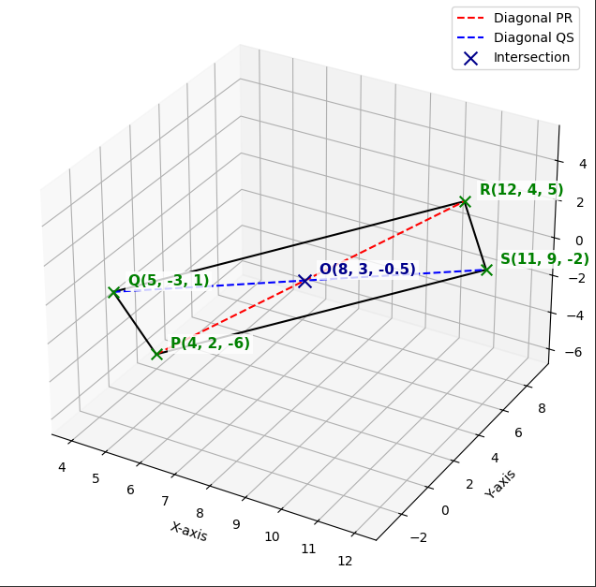
\includegraphics[width=0.5\columnwidth]{figs/graph.png}
\caption*{Parallelogram PQRS with diagonals and intersection)}
\label{fig:graph.png}
\end{figure}
\end{document}